\documentclass[a4paper,11pt]{article}

% Pacotes Principais -----------------------------------------------------------
\usepackage[portuges,brazil]{babel}
\usepackage[utf8]{inputenc}

% Formatação de capítulos ------------------------------------------------------
%\usepackage[Sonny]{fncychap}
%\usepackage{fncychap}
\usepackage{capitulos}

% Figuras e Imagens ------------------------------------------------------------
\usepackage{graphicx}
% Figuras lado a lado
\usepackage{epsfig}
\usepackage{subfigure}

% Utilizar H para inserir as imagens REALMENTE onde eu desejo
\usepackage{float}

% Fontes -----------------------------------------------------------------------
\usepackage[T1]{fontenc}
\usepackage{pslatex}

% Simbolos ---------------------------------------------------------------------
\usepackage{textcomp}
\usepackage{bbding}

% Tabelas ----------------------------------------------------------------------
%\usepackage{multicol}
\usepackage{multirow}
% Colorir a tabela
\usepackage{colortbl}
% Pacote hhline corrige os bugs das linhas que não aparecem com o colortbm
\usepackage{hhline}
% Tabelas com colunas de largura auto ajustável
\usepackage{tabularx}
% Notas de rodapé em tabelas (Pode-se usar o ambiente longtable também -
% Pesquisar exemplo com longtable)
\usepackage{threeparttable}
% Tabelas grandes
\usepackage{supertabular}

% Glossário --------------------------------------------------------------------
\usepackage[portuguese,noprefix]{nomencl}
\usepackage{makeglo}

% Outros pacotes ---------------------------------------------------------------
\usepackage{noitemsep}

% Comentários em bloco
\usepackage{verbatim}

% Hiperlinks
\usepackage{hyperref}

% Orientação de página
\usepackage{lscape}

% utilitários matemáticos
\usepackage{amsmath}
\usepackage{icomma}

% Evita o problema "too many unprocessed floats", colocando os campos
% 'flutuantes' em suas respectivas seções
\usepackage[section]{placeins}

% Referências ------------------------------------------------------------------
\usepackage[abbr]{harvard}	% As chamadas são sempre abreviadas
\harvardparenthesis{square}	% Colchetes nas chamadas
\harvardyearparenthesis{round}	% Parêntesis nos anos das referências
\renewcommand{\harvardand}{e}	% Substituir "&" por "e" nas referências

% Comandos gerais --------------------------------------------------------------
\newcommand{\titulo}{Sistemas de Tempo Real}
\newcommand{\autor}{Diogo Leite Rebouças}

% Configuração da fonte
%\renewcommand{\familydefault}{\sfdefault}

% Margens ----------------------------------------------------------------------
\setlength{\oddsidemargin}{3.5cm}
\setlength{\evensidemargin}{2.5cm}
\setlength{\textwidth}{15cm}
\addtolength{\oddsidemargin}{-1in}
\addtolength{\evensidemargin}{-1in}

\setlength{\topmargin}{2.0cm}
\setlength{\headheight}{1.0cm}
\setlength{\headsep}{1.0cm}
\setlength{\textheight}{22.7cm}
\setlength{\footskip}{1.0cm}
\addtolength{\topmargin}{-1in}

% Glossário --------------------------------------------------------------------
\makeglossary

% Capítulos --------------------------------------------------------------------
% Não aparecer o número na primeira página dos capítulos
\newcommand{\mychapter}[1]{\chapter{#1}\thispagestyle{empty}}
\newcommand{\mychapterstar}[1]{\chapter*{#1}\thispagestyle{empty}}

% Comandos matemáticos ---------------------------------------------------------
% Implicação em fórmulas
\newcommand{\implica}{\quad\Rightarrow\quad} %Meio de linha
\newcommand{\implicafim}{\quad\Rightarrow}   %Fim de linha
\newcommand{\tende}{\rightarrow}

% Fração com parenteses
\newcommand{\pfrac}[2]{\parent{\frac{#1}{#2}}}

% Transformada de Laplace e transformada Z
\newcommand{\lapl}{\pounds}
\newcommand{\transfz}{\mathcal{Z}}

% Sequências
\newcommand{\sequencia}[4]{$#1_{#2}$, $#1_{#3}$, \ldots, $#1_{#4}$}

% Outros ----------------------------------------------------------------------
\newcommand{\chave}[1]{\left\{#1\right\}}
\newcommand{\colchete}[1]{\left[#1\right]}
\newcommand{\parent}[1]{\left(#1\right)}

\newcommand{\rhoagua}{\rho_{\tiny \text{\tiny H}_2\text{\tiny O}}}

\let\D\displaystyle
\newcommand{\reg}{\textsuperscript{\textregistered}}
\newcommand{\soft}{\textit{software}}
\newcommand{\Soft}{\textit{Software}}

% Imagens exportadas pelo gnuplot ----------------------------------------------
\graphicspath{{imgs/eps/}}


\begin{document}

\begin{table}[H]
\centering
\begin{tabular}{cl}
% Primeira Linha
\multirow{7}{*}
{

\includegraphics[width=1.65cm]{imgs/uern}
} & \\
& Governo do Estado do Rio Grande do Norte\\
% Segunda Linha
& Secretaria de Estado da Educação, da Cultural e dos Desportos -- SECD\\
% Terceira Linha
& {\sc Universidade do Estado do Rio Grande do Norte -- UERN}\\
% Quarta Linha
& Pró-Reitoria de Ensino e Graduação -- PROEG\\
% Quinta Linha
& Ciências da Computação -- 1\textordfeminine\ Avaliação (10 pontos)\\
& 
\end{tabular}
\end{table}

\begin{center}
\large
\uline{Expectativa de Respostas}
\end{center}

\section*{Questão 1 (2 pontos)}
Em nossas primeiras aulas, vimos o que seria {\bf sinal} e o que seria {\bf
informação}. Vimos também que qualquer tipo de informação, independentemente de
sua natureza (analógica ou digital) pode ser codificada em uma estrutura de
dados (mídia de representação). Com base nessas informações e no que foi visto
em sala de aula, responda os itens abaixo.

\begin{itemize}
\item[a)] Defina o que é um sinal e o que é informação.
\end{itemize}

Sinais são ondas (físicas/eletromagnéticas) que podem ser transmitidas através
de algum meio físico. A variação de alguma característica desse sinal
(amplitude, frequência, largura de pulsos \ldots) corresponde à codificação da
informação a ser transmitida.

\begin{itemize}
\item[b)] Um sinal analógico com frequência de 4 MHz deve ser digitalizado em um
computador e transferido para outro. Considerando que cada amostra do sinal será
representada com 4 bits, calcule a taxa de transmissão mínima para que não haja
perda de informação.
\end{itemize}

De acordo com o critério de Nyquist, um sinal de 4 MHz deve ser amostrado, pelo
menos, com 2 vezes essa frequência para que não haja problema de {\it aliasing}.
Assim, deverão ser feitas 8 milhões de amostras por segundo (8 MHz) para
garantir a recuperação do sinal original. 

Como cada amostra do sinal é representada com 4 bits, a taxa de transmissão
necessária será de $8 \text{MHz} \times 4 \text{bits} = 32 \text{Mbits/s}$.

\pagebreak

\section*{Questão 2 (2 pontos)}
De acordo com o que foi visto em sala, quando pessoas distintas mencionam o
termo {\bf multimídia}, talvez estejam se referindo a coisas diferentes.
Defina o que é multimídia e cite algumas das facilidades em se utilizar arquivos
multimídia.

\vspace{0.25cm}

Multimídia são todos os programas e sistemas em que a comunicação entre o homem
e o computador se dá através de múltiplos meios de representação da informação
(som, imagem, animações \ldots).

Dentre as facilidades introduzidas pelo uso de recursos multimídia, pode-se
destacar:

\begin{itemize}
    \item Acesso não linear as informações
    \item Consulta e Atualização de informações armazenadas em bases de dados
    \item Criação de material em tempo real a partir de modelos cliente-servidor
ou de instrumentos reais
    \item Simulação de sistemas físicos com diferentes níveis de realismo
\end{itemize}

\pagebreak

\section*{Questão 3 (2 pontos)}
Quando comentamos em sala sobre autoria multimídia, mostrou-se que, do ponto de
vista de ambiente operacional, um sítio é visto como uma coleção de arquivos
organizados em uma estrutura de pastas. Diferencie {\bf sítios estáticos} de
{\bf sítios dinâmicos} e identifique as duas formas em que os {\bf códigos
ativos} podem ser executados.

\vspace{0.25cm}

Sítios estáticos, diferentemente de sítios dinâmicos, são aqueles que não
possuem código ativo, ou seja, que não possuem programas que são ativados a
partir de ações do usuário durante sua navegação. 

Os códigos ativos, podem ser executados no cliente, quando o navegador é o
responsável pela invocação dentro do computador do usuário final, ou no
servidor, quando são executados pelo próprio servidor Web, produzindo
dinamicamente as páginas HTML que serão enviadas para o usuário.
    
\pagebreak

\section*{Questão 4 (2 pontos)}
Vimos em sala de aula que a construção de um produto multimídia deve ser
realizada a partir de um projeto, o qual denominamos de {\bf projeto
multimídia}. Identifique os elementos que devem ser levados em consideração ao
se elaborar um projeto multimídia. Determine também as fases do modelo de {\bf
ciclo de vida} sugerido em sala de aula, explicando sucintamente o significado
de cada uma delas.

\vspace{0.25cm}

Os elementos a serem levados em consideração em um projeto multimídia são:

\begin{itemize}
    \item \uline{Resultado final}, com possíveis resultados intermediários
    \item \uline{Prazo} para execução, com possíveis prazos intermediários
    \item \uline{Orçamento}, com possíveis itens opcionais
    \item \uline{Cliente} contratante ou público que se pretende atingir
    \item \uline{Usuários}, que nem sempre são clientes
    \item \uline{Equipe de desenvolvimento}, com papeis especializados (gerente,
programadores, artistas, escritores, roteiristas \ldots)
    \item \uline{Ciclo de vida}, descrevendo as fases de existência do produto,
desde a concepção até a ausência de suporte pelo fornecedor
\end{itemize}

O modelo de ciclo de vida sugerido é dividido da seguinte forma:

\begin{itemize}
    \item \uline{Ativação}: Equipe desenvolve as ideias do produto a partir de
estimativas preliminares e apresenta a proposta ao cliente
    \item \uline{Especificação}: Definição precisa e detalhada do produto,
custos e prazos
    \item \uline{Desenvolvimento}: Conjunto de atividades que contemplam a
construção e a operação do produto
    \item \uline{Operação}: Utilização do produto pelos usuários finais com
suporte e manutenção do produtor (conforme contrato)
\end{itemize}

\pagebreak

\section*{Questão 5 (2 pontos)}
Sabemos que as cores podem ser representadas através de combinações lineares de
cores básicas, também denominadas de cores elementares ou cores primárias.
Considerando o {\bf modelo de cores RGB} e a representação de imagens no formato
matricial, responda os itens abaixo.

\begin{itemize}
    \item[a)] Explique como se dá a pigmentação dos {\it pixels} em um monitor
CRT convencional.
\end{itemize}

Os monitores CRT permitem o controle direto de três canhões de elétrons. A
velocidade do elétron que sai de cada canhão depende da tensão que é enviada
para ele.

O choque dos elétrons de cada canhão ativa na tela os pigmentos de fósforo
correspondentes a uma das cores primárias. A mistura das ativações irá gerar a
coloração final de cada {\it pixel} de acordo com o sistema aditivo.

\begin{itemize}
    \item[b)] Considere uma matriz de dimensão $M \times N$ tal como mostra a
Fig. \ref{fig:matriz}. Sabendo que cada célula da matriz representa um {\it
pixel} e que cada {\it pixel} é codificado através do modelo RGB com {\bf 1
Byte/cor}, qual será o tamanho do arquivo da imagem ({\bf em KBytes})
representada por essa matriz quando $M = 80$ e $N = 40$?
\end{itemize}

\begin{figure}[H]
\centering
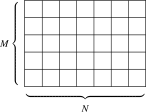
\includegraphics[width=0.3\textwidth]{imgs/matriz}
\caption{Matriz de {\it pixels} utilizada na Questão 5.}
\label{fig:matriz}
\end{figure}

O número total de {\it pixels} será $p = 80 \times 40 = 3.200$. Como cada {\it
pixel} é representado por 3 Bytes (1 Byte/cor), tem-se no total $T = 3.200
\times 3 = 9.600$ Bytes. Como a unidade desejada é dada em KBytes, então,
dividindo T por 1.024, tem-se:

\[
\frac{T}{1.024} = \frac{9.600}{1.024} = 9,375\ \text{KBytes}
\]

\pagebreak

\section*{Questão 6 (1.0 ponto extra)}
Em um sistema de vídeo digital, deseja-se calcular a taxa de transmissão
necessária para realizar a transmissão de um sinal de vídeo sem que haja perda
de informação. Sabe-se que no protocolo de transmissão não há nenhum método de
verificação ou correção de erro. Ou seja, cada bit transmitido errado implicará
em retransmissão total do quadro. 

As especificações do sistema são:

\begin{itemize}
\item Resolução da tela de $640 \times 480$;
\item Quadros utilizam modelo de cor RGBA, sendo 1 Byte/Cor + 1 Byte de
transparência;
\item A taxa de atualização da tela é de 30 quadros/segundo (30 fps).
\end{itemize}

Com base nessas informações, responda:

\begin{itemize}
    \item [a)] Qual será a taxa de transmissão ({\bf em KBytes}) para atender as
especificações acima?
\end{itemize}

O número total de {\it pixels} é $p = 640 \times 480 = 307.200$. Como cada {\it
pixel} é representado por 4 Bytes (1 Byte/cor + 1 Byte de transparência) o
tamanho do quadro será de $T_Q = 307.200 \times 4 = 1.228.800$ Bytes. Como a cada
segundo deverão ser transmitidos 30 quadros, então a taxa de transmissão será:

\[
tx = 1.228.800 \times 30 = 36.864.000\ \text{Bytes/s}
\]

Como se deseja a taxa em KBytes, então:

\[
tx_{MB} = \frac{tx}{2^{10}} = \frac{36.864.000}{1024} = 36.000\ \text{KBps}
\approx 35,156\ \text{MBps}
\]

\begin{itemize}
    \item [b)] Qual é o número de quadros transmitidos em 1 minuto de vídeo?
Qual volume de informação em GBytes?
\end{itemize}

O número de quadros transmitidos em um minuto de vídeo seria o número de quadros
transmitidos a cada segundo vezes sessenta segundos, logo: $N = 30 \times 60 =
1800$ quadros.

Considerando que a cada segundo são gerados $36.864.000$ Bytes de informação,
para 60 segundos, existirão $60 \times 36.864.000 = 2.211.840.000$ Bytes, o que
equivaleria a:

\[
%\stackrel{abc}{\Longrightarrow} % Escrever em cima da seta
2.211.840.000\ \text{Bytes} \xLongrightarrow{\div 1024\ }
2.160.000\ \text{KBytes} \xLongrightarrow{\div 1024\ }
2.109,375\ \text{MBytes} \xLongrightarrow{\div 1024\ }
2,06\ \text{GBytes}
\]

\begin{itemize}
    \item [c)] Supondo que a cada 90 quadros, 1 quadro é perdido (precisa ser
retransmitido), qual será o volume de dados em MBytes que precisará ser
retransmitido na transmissão de 1 minuto de vídeo?
\end{itemize}

Em 1 minuto de vídeo são transmitidos $30 \times 60 = 1.800$ quadros. Como a
cada $90$ quadros, $1$ deve ser retransmitido, então para $1.800$ quadros, serão
retransmitidos $Q_R = 1.80\cancel{0} \div 9\cancel{0} = 20$ quadros.
Considerando que cada quadro representa $1.228.800$ Bytes, tem-se:

\[
T_B = 1.228.800 \times 20 = 24.576.000\ \text{Bytes a serem
retransmitidos}
\]

O que por sua vez, representa:

\[
%\stackrel{abc}{\Longrightarrow} % Escrever em cima da seta
24.576.000\ \text{Bytes} \xLongrightarrow{\div 1024\ }
24.000\ \text{KBytes} \xLongrightarrow{\div 1024\ }
23,4375\ \text{MBytes}
\]

\end{document}
